\chapter{Grundlagen}
\label{cha:grundlagen}

% Abschnitt: Quartettspiel
\section{Grundlagen der Bewertungen und Wartezeitenberechnung}
\label{sec:grundlagen:bewertugnen}

TODO


% Abschnitt: Mobile Plattform
\section{Mobile Plattform Android}
\label{sec:grundlagen:plattforml}

Android ist ein mobiles Betriebssystem, also für Smartphones und Tablets, das von Google entwickelt wurde und auf Linux basiert. Die App-Entwicklung ist geprägt durch einzelne Aktivitäten (ein angezeigter Screen ist eine Aktivität), die miteinander kommunizieren und in ihrer 'Lebenszeit' ein vorgegebenes Zustandmodell \ref{figure:androidZustandsmodell} durchlaufen.

\begin{figure}[htp]
	\centering
  	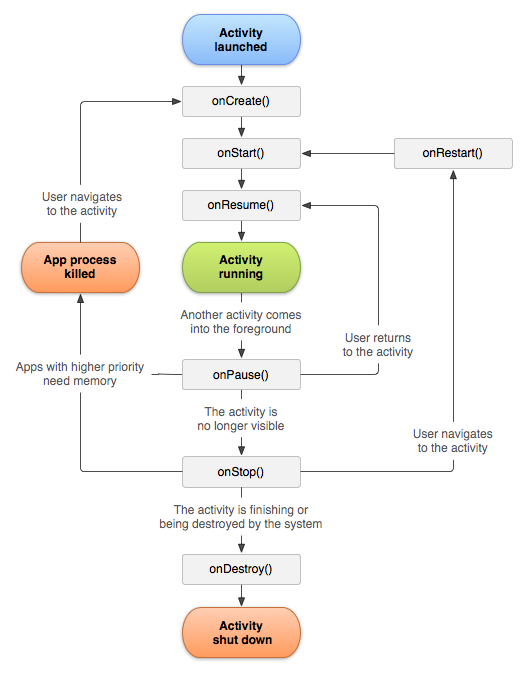
\includegraphics[width=0.4\textwidth]{img/modelle/AndroidZustandsmodell.png}
	\caption{Android Zustandsmodell}
	\label{figure:androidZustandsmodell}
\end{figure}

Dieses Zustandmodell ist auch anfangs einer der Nachteile von Android, da es nicht so leicht zu verstehen ist und uns auch ein paar Probleme bereitet hat. Nachdem wir uns aber im Laufe der App-Entwicklung immer mehr mit Android vertraut gemacht haben, war auch das Modell kein Problem mehr, sondern eher ein Vorteil, da es sehr logisch und durchdacht ist. Eine weitere Schwierigkeit, die während der Entwicklung aufgetreten ist, ist, dass es so viele verschiedene Android-Versionen und Geräte gibt. Da wir unsere App für so viele Versionen wie möglichen entwickeln wollten, kamen deshalb auch mal das ein oder andere Problem auf, wie z. B. dass manche Libraries oder Frameworks erst ab bestimmten Versionen verfügbar sind oder die vielen verschiedenen Geräte alle unterschiedlichen Seiten- und Größenverhältnisse haben.\\
Die Vorteile von Android überwiegen aber auf jeden Fall, vor allem, wenn man sich damit tiefer beschäftigt und eingearbeitet hat. Einer der größten Vorteile ist die sehr gute Dokumentation von Android durch die das Einlesen in die Möglichkeiten und Funktionen recht leicht ist. Auch die weltweite Verbreitung und Beliebtheit von Android ist hier ein Vorteil, da es sehr viele Entwickler gibt und so jedes Problem schon eimal aufgetreten ist und daher auch zu den allermeisten auch Lösungen oder Workarounds bekannt sind.
Außerdem wird Android stetig Weiterentwickelt, weshalb immer mehr möglich ist und der Umgang mit bestimmten Funktionen, wie z. B. der Zugriff auf Gerätefunktionen wie Kamera oder Galerie immer leichter wird.
Weitere Vorteile für uns sind die Vertrautheit mit Java und die Einfachheit von Android Studio.

% Abschnitt: Frameworks
\section{Frameworks}
\label{sec:grundlagen:frameworks}
TODO
Frameworks sind eine Art Gerüst oder Rahmen, die eingesetzt werden um das Programmieren zu vereinfachen und die geschriebenen Zeilen zu verringern.\\
Wir haben in unserer App drei Frameworks als Hilfen genutzt:
\begin{itemize}
\item Picasso: Erlaubt einfaches Handling (z. B. Größentransformationen) von Bildern in oftmals einer Zeile
\item MPAndroidCharts: Ermöglicht die Erstellung von Diagrammen (in unserem Fall Tortendiagramme für die Statistiken)
\item com.github.clans:fab: Ein fancy Menü, das schön ein- und ausgeklappt werden kann
\end{itemize}



















